\documentclass[a4paper]{article}

\usepackage[english]{babel}
\usepackage[utf8]{inputenc}
\usepackage{amsmath}
\usepackage{graphicx}
\usepackage[colorinlistoftodos]{todonotes}
\usepackage{hyperref}
\usepackage{ amssymb }
\usepackage[normalem]{ulem}
\usepackage{amsfonts}
\usepackage{amsmath}
\usepackage{graphicx}
\usepackage{float}
\usepackage{bm}
\usepackage{caption}

\usepackage{amsmath,amsfonts,amssymb}




\title{ML Fundamentals}
\author{Reid Pryzant}
\date{September 3rd, 2015}

\begin{document}
\maketitle

\section{Machine Learning Fundamentals}
Deep learning is a branch of machine learning. In order to build an understanding of deep learning, then, we need background on the basic principles of machine learning. 
\\ \\
\noindent A machine learning algorithm is one that is capable of improving automatically from experience. In most cases, ``experience" in this context means data, but how does an algorithm actually go about learning how to do things? In answering this question, it is advantageous to formalize our discussion. A popular definition of learning in the context of algorithms and code is as follows:
\\ \\
\noindent {\bf Definition:} ``A computer program is said to $learn$ from experience $E$ with respect to some class of tasks $T$ and performance measure $P$, if its performance at tasks in $T$, as measured by $P$, improves with experience $E$" \cite{mitchell}. 
\\ \\
\noindent In other words, when a program is trying to accomplish some task, it measures its performance as it runs. A program $learns$ when its performance on this task improves over time. For example, if a computer program is learning how to play ping pong with a robotic arm, the task is $playing\ ping\ pong$, its performance is measured by its $ability\ to\ win$, and it accrues experience by $playing\ games\ of\ ping\ pong$. 
\\ \\ 
\noindent By this point, we have assembled the needed framework to understand our first machine learning algorithm: $linear\ regression$. It is a simple example that underlines many of the fundamental ideas we will encounter. It is also a good chance to wet our toes with the kind of mathematical thinking we will encounter during our exploration of deep learning. Even if you know what linear regression is, it is valuable and refreshing to reconsider from a machine learning perspective. 
\\ \\
\noindent In the case of linear regression the task is predicting the value of a scalar $y \in \mathbb{R}$ (a number) based on a vector input $\bm{x}\in \mathbb{R}^{n+1}$ (several numbers denoted $x_0,\ x_1,\ x_2,...,\ x_n$ where $x_0 = 1$). This task can be thought of as follows: we have a bunch of observations ($\bm{x}, y$). We assume the $y$'s are generated by a function $f(\bm{x})=y$. We want to learn what $f$ is, so we develop an approximation of $f$ called $\hat{f}$. Note that our $\hat{f}$ will produce approximations of the $y$'s: $\hat{f}(\bm{x}) = \hat{y}$. In a machine learning context, $f$ is often assumed to be a probability distribution that is generating each $y$. $\hat{f}$ maps $\bm{x}$ to $\hat{y}$ by taking a linear combination of $\bm{x}$ and its $parameters$ $\bm{w}$. This means that 
\begin{align*}
\hat{f}(\bm{x}) &= \hat{y} \\
&= \bm{w}^{\intercal} \bm{x} \\
&= \sum_{i = 0}^n w_i x_i \\
&= w_0 + w_1 x_1 + w_2 x_2 + \cdot \cdot \cdot + w_n x_n
\end{align*} 
\noindent where $\bm{w} \in \mathbb{R}^{n+1}$ is a vector of parameters. In a machine learning context, the parameters are known as $weights$. Weights control the behavior of our predictions. Each weight $w_i$ controls how much power the $i^{\mathrm{th}}$ input has in determining the output $\hat{y}$. 
\\ \\
\noindent We now have a good grasp on our task: to produce a mapping of $\bm{x}$'s to $\hat{y}$'s such that $\hat{y} = \bm{w}^{\intercal} \bm{x}$. An example of this might be predicting the probability of a honey bee swarm given some recent weather data and hive demographics. 
\\ \\
\noindent Now we need to be able to track our performance. In linear regression, it makes sense to equate performance with $error$. Good performance is a small error rate, and poor performance is a large error rate. Coming up with a performance measurement, then, is analogous to measuring the error made by our model. 
\\ \\
\noindent A first attempt at defining the error $E$ might simply be the difference between the prediction of our model and the value we are trying to predict:
\begin{align*}
E(\bm{x}) &= f(\bm{x}) - \hat{f}(\bm{x}) \\
&= y - \hat{y}
\end{align*}
\noindent The problem with this is that if $\hat{y} > y$, then $E$ will be negative. This doesn't make sense (what does a negative error mean?), so we might redefine a new error, $E'$, that takes the absolute value of this difference
\begin{align*}
 E'(\bm{x}) &= \vert f(\bm{x}) - \hat{f}(\bm{x})\vert \\
 &= \vert y - \hat{y} \vert
 \end{align*}
\noindent This works, but our intuition tells us that the more wrong a prediction is, the worse its error should be. This leads us to the $squared\ error$ measure, one we will use later in our discussion of neural networks:
\begin{align*}
E''(\bm{x}) &= ( f(\bm{x}) - \hat{f}(\bm{x}))^2  \\
&= ( y - \hat{y} )^2 
\end{align*}
\noindent Now that we have a task and a performance measurement, we need to think about what $experience$ means in the context of regression. Experience is the same thing as data. More experience is more data. The data come in two types. The first, $\bm{X}^{m +1 \times n}$, is a special matrix called the $design\ matrix$. It consists of a list of $n$ $observations$ $\bm{x}_1$, $\bm{x}_2$, ..., $\bm{x}_n$. Each observation is a single vector or data point. Observations consist of $m$ $attributes$ (1, $x_1$, $x_2$, ..., $x_m) \in \bm{x}$. In a graphical interpretation, each $x_i \in \bm{x}_k$ is a coordinate for the $i^{\mathrm{th}}$ dimension for data point $k$. 
\[
\bm{X} = \begin{bmatrix}
 \bm{x_1} & ... & \bm{x_n}
 \end{bmatrix}
=\begin{bmatrix}
1 & 1 &...&1 \\
x_{11} & x_{12} & ... & x_{1n} \\
...& ... &... & ...\\
x_{m1} & x_{m2}& ...& x_{mn}
\end{bmatrix}
\]
The second data matrix is $\bm{y}$. This is a vector of regression targets -- things we are trying to predict. 
\\ \\
\noindent We can expand our definition of error so that it takes this data into account. The result, $mean\ squared\ error$ ($MSE$), is an average of all the $E''$ values each $\bm{x}_i$:
\[ MSE = \frac{1}{n}\sum_{i = 1}^n \bigg( f(\bm{x}_i) - \hat{f}(\bm{x}_i)\bigg)^2 \]
\noindent Notice that the format our linear regression problem has taken is now the same as the kinds of problems machine learning algorithms try to solve. We have a bunch of stuff to be done (predict $\hat{y}$'s from all of the $\bm{x}_i$'s) and a bunch of stuff that's already done ($y_i$'s for each $\bm{x}_i$). All that remains is to show the model this data and $teach$ it how to improve its predictions.
\\ \\
\noindent When we say $learn\ from\ data$, we mean leveraging our experience to improve performance. With regards to linear regression this means using our data ($\bm{X}$ and $\bm{y}$) to find the weights $\bm{w}$ that perform the best (produce the smallest $MSE$). This process is called $optimization$. 
\\ \\
\noindent There are many ways to optimize for $\bm{w}$, each with their own interpretation. My personal favorite comes from linear algebra. To start, lets put the task at hand into matrix notation. We are trying to solve for
\begin{align*}
\hat{\bm{y}} &= \bm{X}^\intercal \bm{w} \\
\begin{bmatrix}
\hat{y}_1 \\
\hat{y}_2 \\
\cdot\cdot\cdot\\
\hat{y}_n 
\end{bmatrix} &=
\begin{bmatrix}
1 &x_{11}&...&x_{1m}\\
...& ... &... & ...\\
1 & x_{n1}& ...& x_{nm}
\end{bmatrix}
\begin{bmatrix}
w_0 \\
w_1 \\
... \\
w_m
\end{bmatrix}
\end{align*}
so that our choice for $\bm{w}$ produces the optimal $\bm{\hat{y}}$. This can be rewritten as solving 
\begin{align*}
\bm{y} &= \bm{X}^\intercal \bm{w} + \bm{\epsilon}\\
\begin{bmatrix}
y_1 \\
y_2 \\
\cdot\cdot\cdot\\
y_n
\end{bmatrix} &= 
\begin{bmatrix}
1 &x_{11}&...&x_{1m}\\
...& ... &... & ...\\
1 & x_{n1}& ...& x_{nm}
\end{bmatrix}
\begin{bmatrix}
w_0 \\
w_1 \\
... \\
w_m
\end{bmatrix}
+ \begin{bmatrix}
\epsilon_1 \\
\epsilon_2 \\
... \\
\epsilon_n
\end{bmatrix}
\end{align*}
\noindent where the individual $\epsilon_i$'s are the $error\ terms$ for each observation $i$:
\begin{align*}
\epsilon_i &= (y_i - \hat{y}_i)^2
\end{align*} 
\noindent Optimizing $\hat{f}$, then, becomes the task of choosing a $\bm{w}$ such that the mean of all $\epsilon_i$'s is minimized. 
\\ \\
\noindent Now for the fun stuff. Remember that each vector has a visual interpretation as a point in a coordinate system. The entire $\bm{y}$ and $\bm{\hat{y}}$ vectors are merely points in $n$-dimensional space (because $\vert \bm{y}\vert = \vert\bm{\hat{y}}\vert = n$). Each observation is a point in $m+1$ dimensional space (because each$\ \bm{x}_i \in \bm{X}$ has length $m+1$). Running data points through $\hat{f}$ is equivalent to taking a $linear\ combination$ of each $\bm{x} \in \bm{X}$ because we can only perform linear operations on each observation: we can multiply attributes by weights and sum the results. This means that the only $\bm{\hat{y}}$'s that are possible are those reachable by taking different linear combinations of our $\bm{x}$'s. All of the possibilities for $\bm{\hat{y}}$, then, create a region within our $m+1$ dimensional space. This region is known as the space $spanned$ by $\bm{X}$. 
\\ \\
\noindent The process of optimizing $\bm{w}$ now has a nice visual interpretation to it. Because $\bm{y}$ exists in $n$ dimensions and the space spanned by $\bm{X}$ exists in only $m+1$ dimensions, we need to $project$ $\bm{y}$ into this lower-dimensional world (note that we are assuming $n > (m +1)$). We do this by selecting the $\bm{w}$ that makes $\bm{\hat{y}} = \bm{X}^{\intercal} \bm{w}$ as close as possible to $\bm{y}$!
\begin{figure}[H]
  \centering
  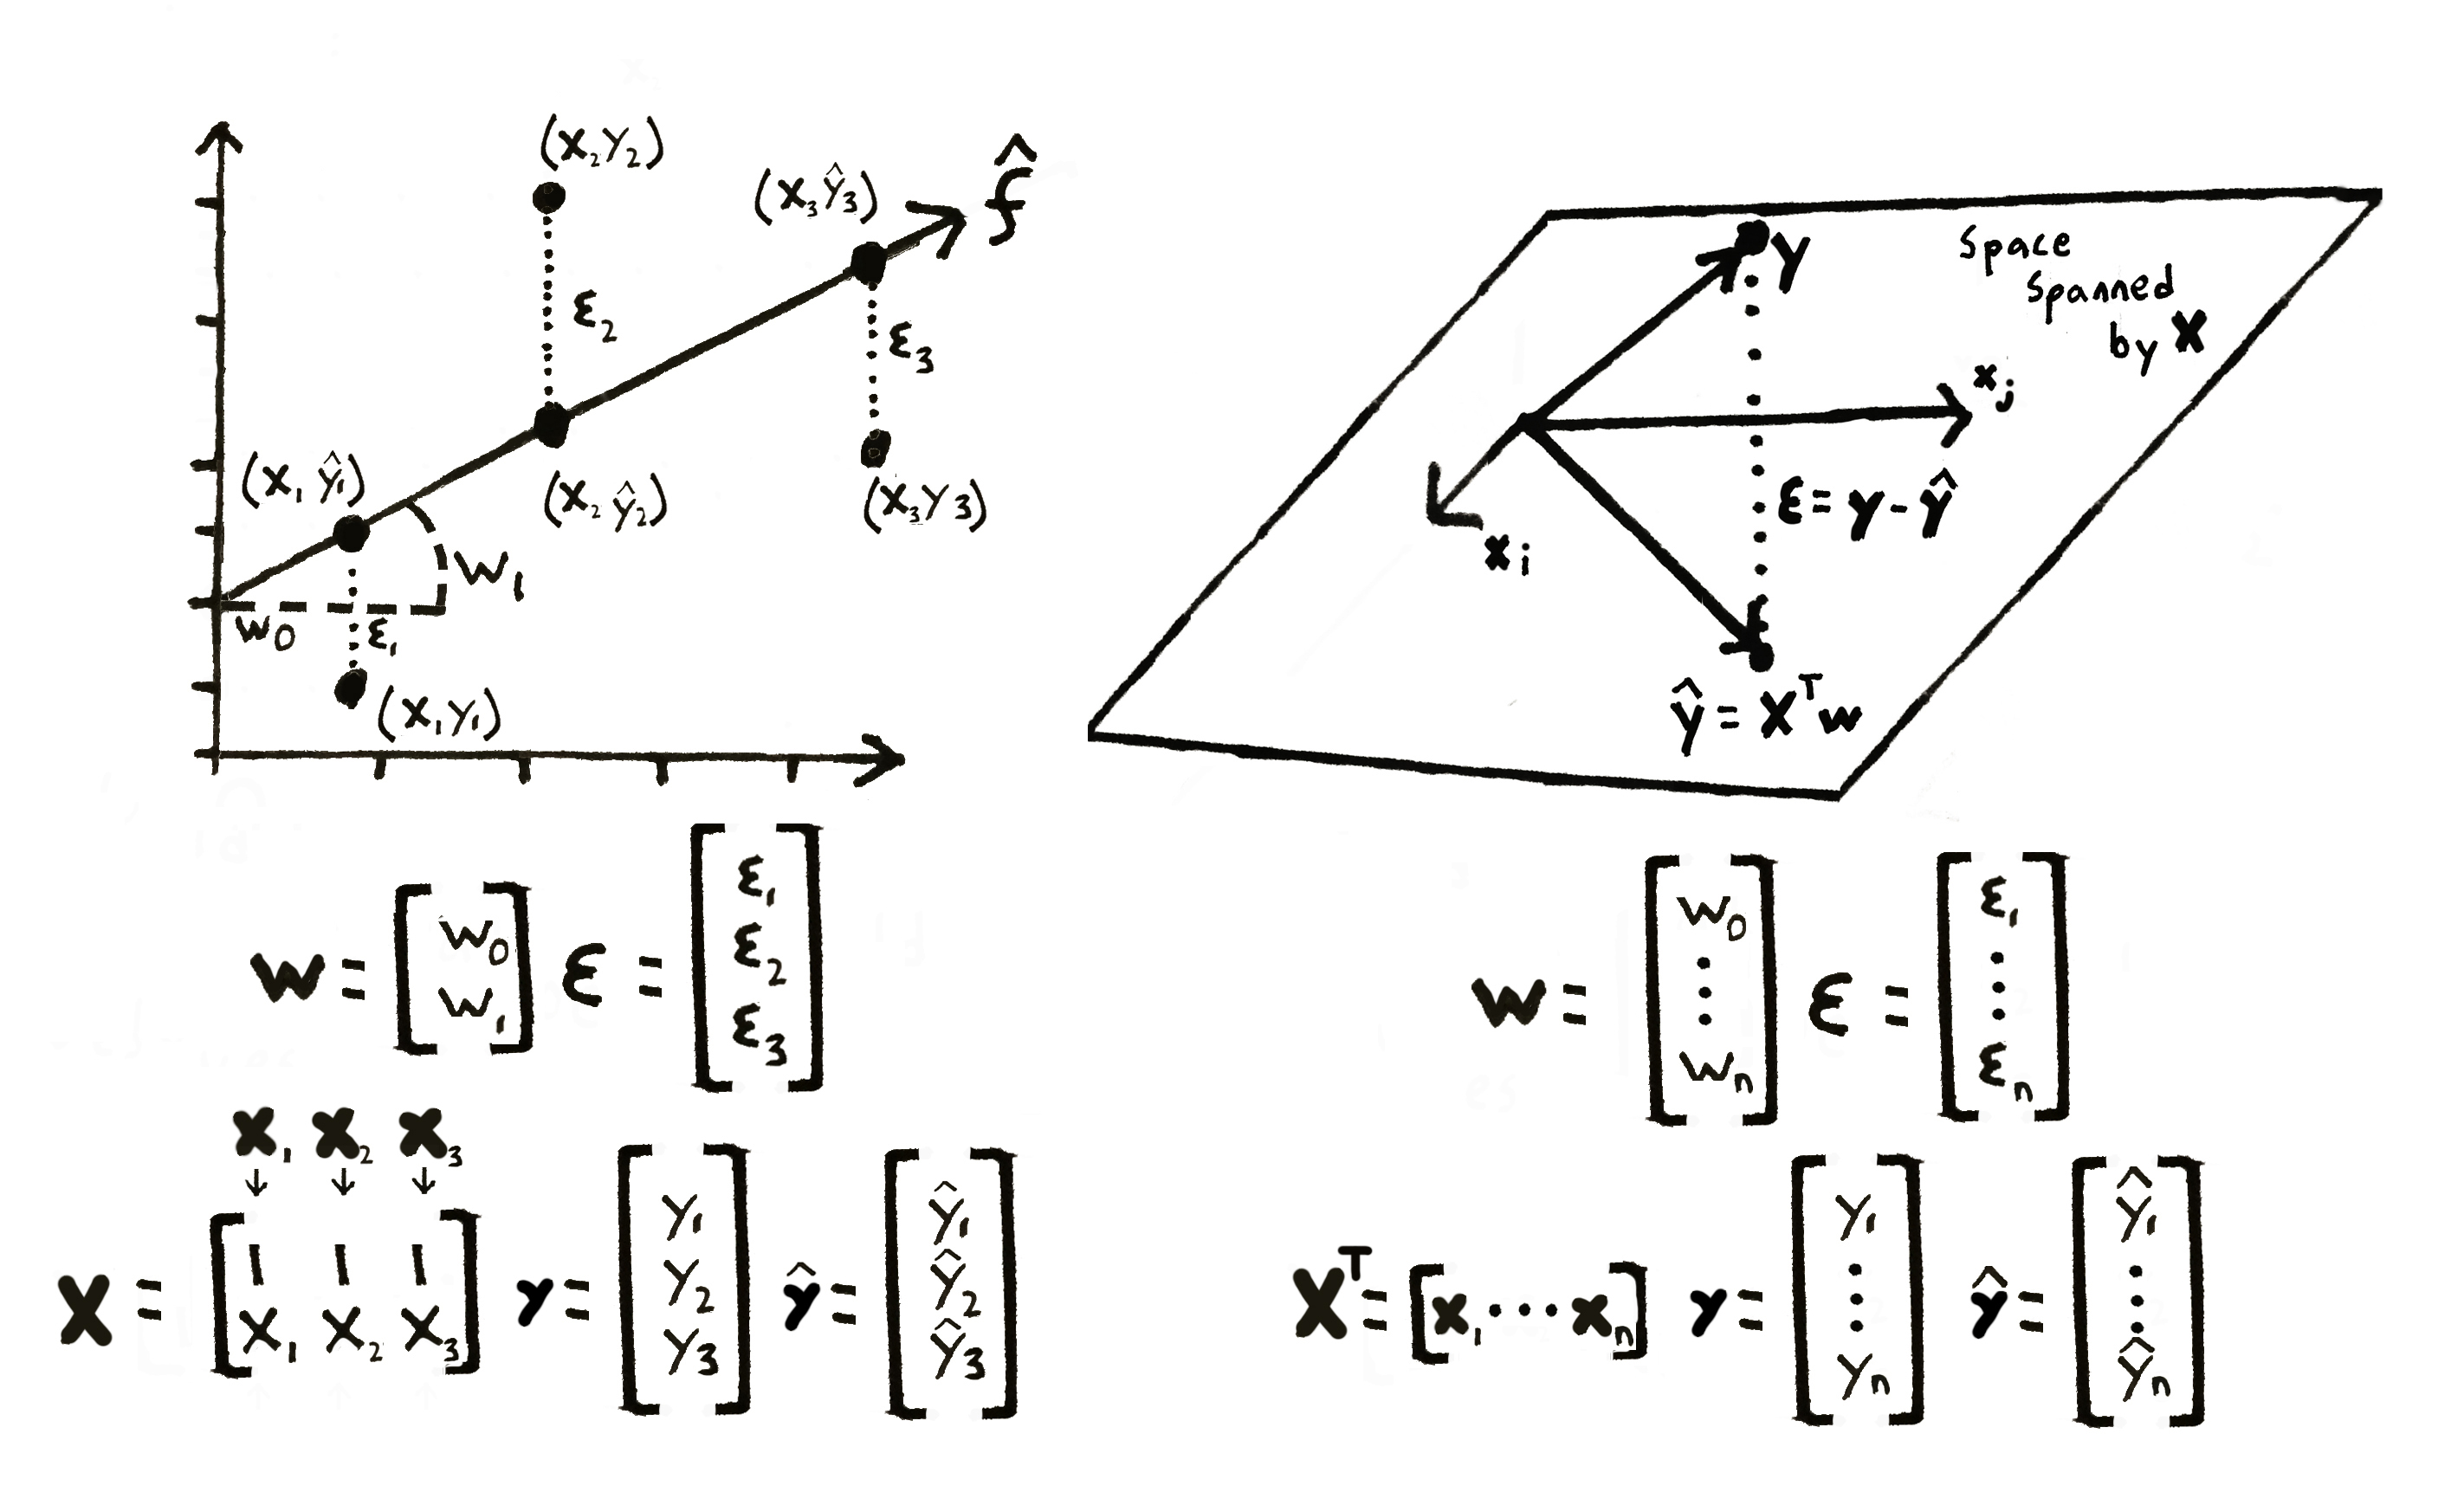
\includegraphics[width=6in]{figures/chap1/regression_projection}
  \caption{Two interpretations of linear regression. To the {\it left} is the coordinate-space interpretation of regression with 1-dimensional inputs. To the $right$ is the vector-space interpretation of regression with high dimensional inputs.}
\end{figure}
\noindent By selecting a $\bm{w}$ in this way, our algorithm is learning how to improve (produce better predictions that minimize error) by using experience, or data. 
\\ \\
\noindent This concludes our discussion of linear regression. The core idea that is at the heart of this algorithm, improving with experience, is one that is central to deep learning and indeed all of machine learning.




\begin{thebibliography}{50}

\bibitem{mitchell}
Mitchell, Tom M. $Machine\ Learning.$ New York: McGraw-Hill, 1997. Print.


\end{thebibliography}

\end{document}
